\documentclass{beamer}

\usepackage{listings}
\usepackage[utf8]{inputenc}
\usetheme{default}

%% set colours
\definecolor{atugreen}{HTML}{005b5e}
\setbeamercolor{title}{fg=atugreen}
\setbeamercolor{frametitle}{fg=atugreen}
\setbeamercolor{section in toc}{fg=atugreen}
\setbeamertemplate{section in toc}{\inserttocsectionnumber.~\inserttocsection}

\title{GLM Model Selection and Validation}
\author{Cóilín Minto, Olga Lyashevska}
\date{July 15\textsuperscript{th} 2022}
\institute{Marine and Freshwater Research Centre\\ Atlantic Technological University \\ Galway, Ireland}
%% logo
\titlegraphic{
    
\includegraphics[width=4cm]{figures/ATU-Logo-Full-RGB-Green-big.jpg}
}

\AtBeginSection[]{
\begin{frame}[noframenumbering, plain]
\frametitle{Outline}
\tableofcontents[currentsection]
\addtocounter{page}{-1}
\end{frame}
}

\begin{document}

\begin{frame}
 \maketitle
\end{frame}

\section{Model Selection}

% \begin{frame}
%  \frametitle{Describe these data}
%  \begin{center}
%     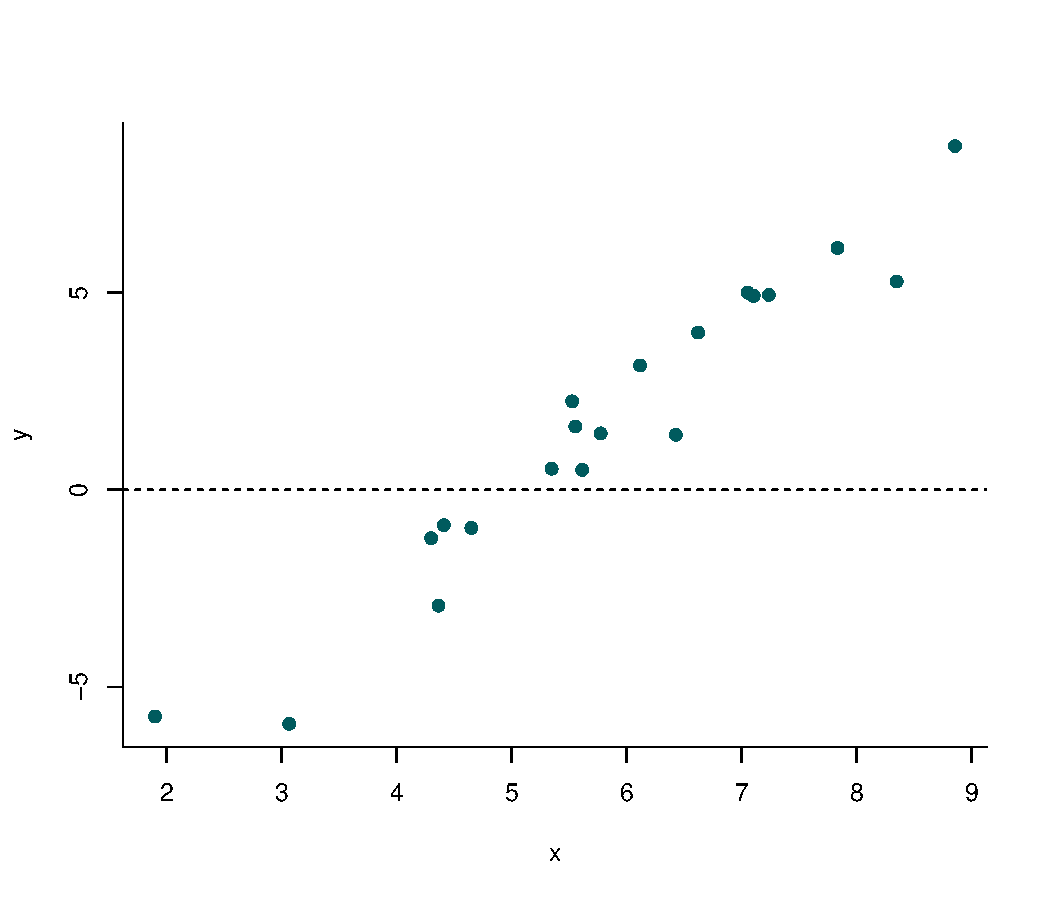
\includegraphics[width=10cm]{figures/continuous_y_0.pdf}
%  \end{center}
% \end{frame}

\begin{frame}{All models are wrong but some are useful}{}

\begin{itemize}
\item Statistical models are mathematical approximations to reality that represent the important features of data for the
task at hand.
\pause
\item The purpose of a statistical model effects how it is developed: prediction versus interpretation (association not cause-effect)
\pause
\item There are numerous predictors that could be chosen. How do we choose a statistical model? Statistical models are based on underlying theory, or from an understanding of the biological features, and are built with this knowledge in mind. 
\end{itemize}

\end{frame}

\begin{frame}{Criteria for model selection}{}
An adequate statistical model balances two criteria:
\begin{itemize}
\item \textbf{Accuracy:} The model should accurately describe both the systematic (how the mean response changes as the explanatory variables change) and the random  (the variation of the data about the mean) component;  
\pause
\item \textbf{Parsimony:} The model should be as simple as possible. The simplest accurate model is the preferred model. Complex models may fit the given data well but usually do not generalize well to other data sets (over-fitting);
\end{itemize}
\end{frame}

%%\begin{frame}[fragile]
%%  \begin{lstlisting}
%%fib <- function(n) {
%%  if (n < 2)
%%    n
%%  else
%%    fib(n - 1) + fib(n - 2)
%%}
%%   \end{lstlisting}
%%\end{frame}
%
\begin{frame}{Why model selection?}

\begin{enumerate}
	\item The deviance of the model (reciprocally the likelihood and the  $R^{2}$) always decreases (increases) with the inclusion of more predictors – no matter whether they are significant or not.
		\pause
	\item The excess of predictors lead to a larger variability in the estimation of the model which results in lower precision.
		\pause
	\item Multicollinearity may hide significant variables, change the sign of them, and result in an increase of the variability of the estimation.
%	\item Roughly speaking, the BIC is consistent in performing model-selection, and penalizes more the complex models when compared to AIC and LOOCV.
\end{enumerate}
\end{frame}

\begin{frame}
\frametitle{Comparing 2 nested models}
	\begin{equation}
	\mu_{A} =\beta_{0}+ \ldots + \ldots + \beta_{3} 
	\end{equation}
	\begin{equation}
	\mu_{B} =\beta_{0}+ \beta_{1} + \beta_{2} + \beta_{3} 
	\end{equation}
	\pause

Model (1) is nested in Model (2), since Model (1) is a special case of Model (2) obtained by setting $\beta_{1}$ and $\beta_{2}$ to 0.  In comparing these models, we wish to know whether the more complex model is necessary.
\end{frame}

\begin{frame}[fragile]
\frametitle{Stepwise selection}
\begin{itemize}
\item We can look at AICs:
\begin{lstlisting}
AIC(mod1)
\end{lstlisting}
Lower AIC values gives better model.

\item Or through \textit{MASS::stepAIC}
\begin{lstlisting}
MASS::stepAIC(mod2, trace = FALSE)
\end{lstlisting}

\item Compare 2 nested models 
\begin{lstlisting}
anova(mod1, mod2)
\end{lstlisting}

\item Dredge 
\begin{lstlisting}

\end{lstlisting}
\end{itemize}
\end{frame}



\section{Model Validation}

\begin{frame}{Diagnostics} 
The estimation and inference from the regression model depends on several assumptions.
There are three categories:
\begin{itemize}
\item \textbf{Error}: 
We assume that $\epsilon \sim N(0, \sigma^{2})$ or in other words, that the errors are normally distributed with mean zero and equal variance $\sigma^2$. 
\item \textbf{Model:} 
We assume that the model is correct

\item \textbf{Unusual observations:} can have a dramatic effect and need to be detected!
\end{itemize}
\end{frame}


\begin{frame}{Checking error assumptions} 
\begin{itemize}
	\item independent for different data values (name?, example?);
	\item have mean zero; 
	\item have constant variance (name? example?);
	\item follow a Normal distribution.
\end{itemize}

\pause
\vspace{1cm}
Which assumption is the most important?
\end{frame}


\begin{frame}{Relative importance of assumptions}
\begin{itemize}
	\item Independence of the errors (zero autocorrelation) is the most important and also most difficult to accommodate when fails (observations are close in time or space);
	\pause
\item Constant variance (homoscedasticity) is intermediate, in that nonconstant variance (heteroscedasticity) can have a substantial effect on inferences, but can also be accommodated in many situations.
	\pause
\item Normal distribution is the least important assumption, especially for large sample size.
Normal distribution of errors is needed for inference. Some models depend more on normality than others.

\end{itemize}
\end{frame}



\begin{frame}{Violation of assumptions}

Violation of assumptions can lead to bias in:

\begin{itemize}
	\item regression coefficients
	\item standard errors
	\item confidence intervals
	\item significance tests  
\end{itemize}
	\vspace{1cm}
\pause The quality of inference depends on how well the errors $\epsilon_{i}$ conform to our assumptions.
\pause  We do not observe the errors. So how do we check these assumptions?
\pause The closest we can get to the errors are residuals $r_{i}$.
\end{frame}

\begin{frame}{Residuals}

What exactly are residuals?
\pause
\vspace{1cm}

Regardless the structure and complexity of the model the raw residuals $r_{i}$ are simply the differences between the data $y_{i}$ and the fitted value $y_{i}$ 

\end{frame}

\begin{frame}{Residuals}

\begin{center}
     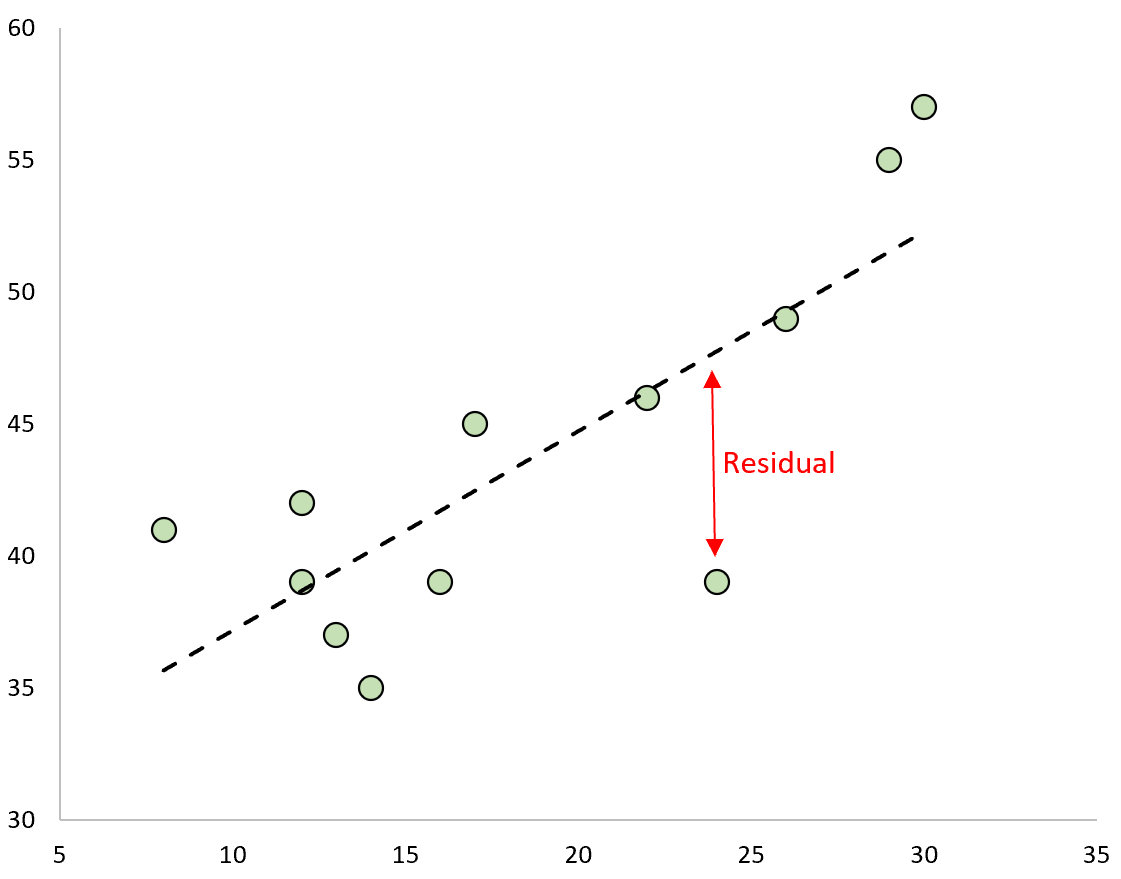
\includegraphics[width=10cm]{../tex/figures/residuals1-1.png}
\end{center}

\end{frame}



\begin{frame}{Heteroscedasticity}
	\begin{itemize}
		\item Plot the residuals $r_{i}$ against the fitted values $y_{i} - r_{ij}$ 
		\item If the variance is constant, the vertical spread of the points will be about the same. 
		\item Nonconstant variance is revealed as a pattern in the spread of the residuals.
	\end{itemize}
\end{frame}

\begin{frame}{Heteroscedasticity}

\begin{center}
     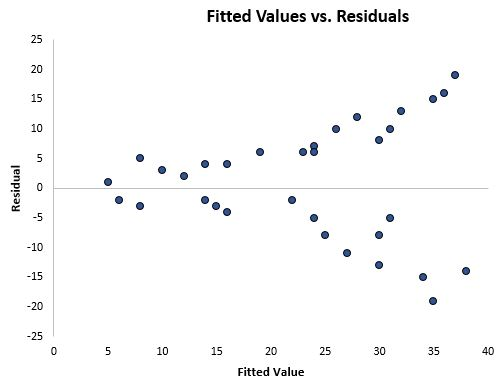
\includegraphics[width=10cm]{../tex/figures/heteroscedastisity.jpg}
\end{center}

\end{frame}



\section{Principles for improved statistical ecology}

\begin{frame}{Four principles for improved statistical ecology}{ISEC 2022, Session 18. Statistical Theory. Gordana Popovic}

\begin{enumerate}
    \item First define a focused research question, then plan sampling and analysis to answer it; 
    \item Develop a model that accounts for the distribution and characteristics (dependencies) of your data;
    \item Emphasise effect sizes to replace statistical significance (p-values) with ecological relevance;
    \item Report you methods and finding in sufficient detail so that your research is valid and reproducible;
\end{enumerate}
\end{frame}

\begin{frame}

\begin{itemize}
	\item Cleasby, I. R., and Nakagawa, S. (2011). Neglected biological patterns in the residuals: A behavioural ecologist’s guide to co-operating with heteroscedasticity. Behavioral Ecology and Sociobiology, 65(12), 2361–2372. http://www.jstor.org/stable/41414703
\end{itemize}
\end{frame}
\end{document}
